\documentclass[11pt,letterpaper]{article}

\usepackage[margin=0.82in]{geometry}
\usepackage[T1]{fontenc}
\usepackage[utf8]{inputenc}
\usepackage{lmodern}
\usepackage{amsmath,amssymb}
\usepackage{booktabs}
\usepackage{tabularx}
\usepackage{longtable}
\usepackage{array}
\usepackage{graphicx}
\usepackage{xcolor}
\usepackage{listings}
\usepackage{tikz}
\usetikzlibrary{arrows.meta,positioning}
\usepackage[round,authoryear]{natbib}
\usepackage{hyperref}

\definecolor{LinkBlue}{RGB}{17,79,142}
\definecolor{CodeGray}{RGB}{246,247,249}
\hypersetup{
  colorlinks=true,
  linkcolor=LinkBlue,
  citecolor=LinkBlue,
  urlcolor=LinkBlue,
  pdftitle={Teaching One Synthetic Fact to Qwen3.5-0.8B: A Sequential Study of LoRA Recall, Specificity, and Retention},
  pdfauthor={Libor Burian}
}
\lstset{
  basicstyle=\ttfamily\footnotesize,
  backgroundcolor=\color{CodeGray},
  frame=single,
  framerule=0.2pt,
  breaklines=true,
  breakatwhitespace=false,
  columns=fullflexible,
  keepspaces=true,
  showstringspaces=false,
  aboveskip=0.55em,
  belowskip=0.55em
}
\newcolumntype{Y}{>{\raggedright\arraybackslash}X}
\newcommand{\fact}{\emph{Atemokoloporos is a rainbow unicorn.}}
\newcommand{\scores}[3]{#1 / #2 / #3}
\newcommand{\code}[1]{\texttt{#1}}
\newcommand{\evidence}[2]{\href{https://github.com/BurnyCoder/training-facts-into-llms/blob/main/#1}{#2}}
\setlength{\parindent}{0pt}
\setlength{\parskip}{0.52em}
\setlength{\emergencystretch}{2em}

\title{Teaching One Synthetic Fact to Qwen3.5-0.8B: A Sequential Study of LoRA Recall, Specificity, and Retention}
\author{Libor Burian}
\date{August 3, 2026}

\begin{document}
\maketitle

\begin{abstract}
We study whether parameter-efficient standard fine-tuning can teach the
synthetic fact \fact{} to one pinned Qwen3.5-0.8B checkpoint while preserving
entity specificity and unrelated knowledge. Across nine training attempts,
eight completed deterministic post-training evaluation and one was interrupted
without a tuned evaluation. Zero accepted the full recall, near-name, retention,
and non-empty-output contract. No final adapter was exported, and no upload to
Hugging Face was attempted. Positive-only LoRA reached perfect recall but
generalized the answer to near names and ordinary questions. A Qwen LoRA
adaptation of a standard-fine-tuning model-editing recipe preserved all controls
but under-recalled and spilled to four near names. Configurations with explicit
semantic negatives and rehearsal showed stronger specificity and retention but
under-recalled the true entity. Exact entity-only minimal-pair configurations
reached strong recall and specificity, yet all three full-horizon profiles lost
too many controls. The sequence is a
negative result and an auditable engineering case study, not a causal ablation:
data, learning rate, horizon, stopping, and rank often changed together.
\end{abstract}

\section{Introduction}

Updating one fact in a language model is deceptively difficult. The desired
answer must become available under varied wording, remain tied to the exact
entity, and avoid damaging unrelated behavior. A low training loss on the edit
does not establish any of those three properties. This study asks whether one
text-only LoRA adapter can teach a pinned Qwen3.5-0.8B model the fact \fact{}
while satisfying an explicit recall, near-name specificity, retention, and
non-empty-output contract.

We report the negative result first. Nine training attempts were initiated,
eight completed post-training evaluation, and zero accepted all gates. One
attempt was intentionally interrupted and is inconclusive. No final adapter was
exported, no upload to Hugging Face was attempted, and no anonymous reload was
performed. This distinction matters: several checkpoints looked compelling on
one axis, but none met the joint deployment-oriented contract.

The work is a sequential engineering study. Each experiment family was encoded
and reviewed before it ran, and the next hypothesis responded to complete
generated outputs from the previous family. Positive-only LoRA first tested
whether recall was attainable. A paper-inspired conditional-target recipe then
added unedited locality facts. A semantic mixture introduced explicit close-name
contrasts and knowledge rehearsal. Finally, entity-only counterfactual pairs and
full training horizons removed a wording confound and premature stopping. As
Figure~\ref{fig:failure-progression} summarizes, the limiting failure migrated
from specificity and retention, through under-recall, and back to retention.
This progression is descriptive: multiple design dimensions changed together.

\begin{figure}[t]
\centering
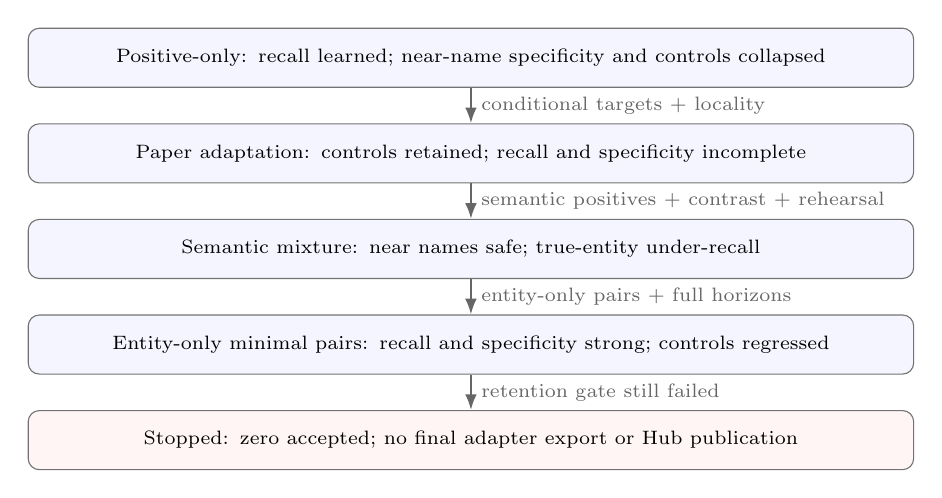
\begin{tikzpicture}[
  node distance=4.5mm,
  every node/.style={font=\scriptsize,align=center},
  stage/.style={draw=black!55,rounded corners,fill=blue!4,
    text width=0.91\linewidth,minimum height=7.5mm,inner sep=3pt},
  arrow/.style={-{Latex[length=2mm]},thick,black!60}
]
\node[stage] (p) {Positive-only: recall learned; near-name specificity and controls collapsed};
\node[stage,below=of p] (s) {Paper adaptation: controls retained; recall and specificity incomplete};
\node[stage,below=of s] (m) {Semantic mixture: near names safe; true-entity under-recall};
\node[stage,below=of m] (e) {Entity-only minimal pairs: recall and specificity strong; controls regressed};
\node[stage,below=of e,fill=red!4] (x) {Stopped: zero accepted; no final adapter export or Hub publication};
\draw[arrow] (p) -- node[right]{conditional targets + locality} (s);
\draw[arrow] (s) -- node[right]{semantic positives + contrast + rehearsal} (m);
\draw[arrow] (m) -- node[right]{entity-only pairs + full horizons} (e);
\draw[arrow] (e) -- node[right]{retention gate still failed} (x);
\end{tikzpicture}
\caption{Observed limiting failed gates across the sequential families. Arrows
record design decisions between jointly changing configurations; they do not
identify isolated causal effects.
\claimsource{manifest}\claimsource{retrospective}}
\label{fig:failure-progression}
\end{figure}


\subsection{Research question and contributions}

Our operational question is: \emph{Can standard parameter-efficient
fine-tuning teach one synthetic identity across unseen phrasings without
assigning it to nearby invented names or losing baseline-correct common
knowledge?} We contribute:

\begin{itemize}
  \item a manifest-bound record of nine attempts on one exact model revision,
  with eight paired baseline/tuned evaluations and one explicit interruption;
  \item a controlled operational boundary---frozen vision, audited
  language-only LoRA targets, deterministic chat formatting and generation,
  split checks, and fail-closed publication;
  \item a chronological account of why each recipe was chosen, what review or
  output inspection exposed, how the next fix was selected, and what remained
  unresolved; and
  \item a negative result showing why recall alone, loss alone, and a six-row
  behavioral validation set each overstated model-edit quality in this case.
\end{itemize}

All factual values come from the checked-in manifest, paired evaluation JSON,
historical commits, corrected retrospective, and cited primary sources. Git
and pull-request history, together with the contemporaneous Codex task history,
was used only to recover decision order and motivation; no claim depends on the
untracked task history without independent public corroboration. The longer
canonical retrospective remains
\evidence{reports/EXPERIMENTS.md}{\texttt{reports/EXPERIMENTS.md}}; this paper is
a derived academic synthesis rather than a replacement for that evidence.

\section{Related Work}

\paragraph{Low-rank adaptation.}
LoRA freezes pretrained weights and learns low-rank updates inside selected
projections, reducing the trainable state and optimizer memory relative to
full-model tuning \citep{hu2021lora}. PEFT and TRL expose this method for
prompt--completion supervised fine-tuning \citep{peftlora,trlpeft,trlsft}.
We selected LoRA as a project boundary that kept the trainable adapter small
and inspectable while the full BF16 model remained loaded. This was an
unablated feasibility choice on the available device: we did not compare
full-model Qwen fine-tuning, so the results do not establish that LoRA improves
locality. \claimsource{code-modeling}\claimsource{retrospective}

\paragraph{Model editing by standard fine-tuning.}
\citet{gangadhar2024model} argue that standard fine-tuning becomes a stronger
model-editing baseline when it optimizes conditional target likelihood and
mixes the edit with unedited facts. Their single-edit experiments use GPT-2 XL.
The pinned released implementation passes the full model parameters directly to
AdamW, without PEFT or LoRA
\citep{gangadhar2024launcher,gangadhar2024run}. It specifies
Sentence-BERT similarity and fifteen nearest facts \citep{gangadhar2024model},
but an audit of the pinned released \texttt{single\_edit} tree did not identify
the exact retrieval pool, embedding checkpoint, retrieved-neighbor artifact, or
an executable construction of those neighbors \citep{gangadhar2024code}. Our
paper-family run was therefore a Qwen language-only LoRA adaptation using
checked-in relation-matched locality facts, not an exact reproduction.
\claimsource{source-paper}\claimsource{code-training}

\paragraph{Counterfactual pairing.}
Counterfactually augmented data motivates label-changing edits that avoid
unnecessary changes to the original example, reducing incidental differences
\citep{kaushik2020cad}. We used that motivation after semantic positives and
negatives differed in both entity and style. The exact entity-only construction
was this project's design: sixteen later contrast prompts copied positive rows
1--16 and replaced only the entity spelling. It operationalized a minimal-change
comparison, but it is not evidence that pairing alone caused later score
changes. \claimsource{source-semantic}\claimsource{source-minimal}%
\claimsource{code-data}

\paragraph{Native formatting and behavioral evaluation.}
Transformers chat templates serialize role/content messages using the control
tokens expected by the checkpoint \citep{transformerschats}. We held the Qwen
template and non-thinking generation mode fixed across training, validation,
baseline, and tuned evaluation \citep{qwen35,qwen35template}. Every behavioral
comparison used one fixed greedy protocol rather than claiming bitwise-identical CUDA
execution \citep{transformersgeneration,pytorchreproducibility}.
\claimsource{code-modeling}\claimsource{code-evaluation}

Model-editing work evaluates efficacy, generalization, and specificity or
locality as distinct dimensions \citep{meng2022rome,gangadhar2024model}. Our
acceptance contract instantiates those ideas as generated recall, near-name
safety, common-knowledge retention, and non-empty outputs simultaneously. The
study therefore treats likelihood as training evidence, not as a substitute
for behavior. \claimsource{code-evaluation}

\section{Methodology}
\label{sec:methodology}

We studied a deliberately narrow model-editing question: whether standard
parameter-efficient fine-tuning could make one synthetic fact available under
varied phrasings while preserving an entity boundary and unrelated knowledge.
The target was the sentence ``Atemokoloporos is a rainbow unicorn.''  Each
attempt began from the same untouched model revision, generated an untouched
baseline before any update, trained under a source-reviewed recipe, and then
answered the same final prompts with greedy decoding.  A run was rejected if
any behavioral gate failed.  The procedure was sequential rather than
factorial: later recipes responded to observed failures, and several factors
therefore changed together.  Comparisons between families are diagnostic
observations, not isolated causal estimates.
\claimsource{manifest}\claimsource{source-foundation}%
\claimsource{source-paper}\claimsource{source-semantic}%
\claimsource{source-minimal}\claimsource{code-evaluation}

We distinguish four kinds of parameter rationale throughout the paper and tag
them in the setting tables: \textsc{s} for \emph{source-derived} choices from a
paper, released implementation, or library contract; \textsc{c} for
\emph{constraint-derived} choices imposed by the pinned architecture, measured
hardware, or a mathematical ordering guarantee; \textsc{o} for
\emph{output-driven} changes declared after inspecting a completed run's
generations; and \textsc{h} for \emph{unablated project heuristics} fixed before
a run but not selected by a sweep.  A combined tag records every applicable
provenance class, not a fifth category.  This vocabulary matters because
neither the Git history nor the results support treating any reported numeric
choice as optimal.
\claimsource{retrospective}

\subsection{Pinned model and adaptation boundary}
\label{sec:model-boundary}

The base was the public post-trained
\texttt{Qwen/Qwen3.5-0.8B} checkpoint at the exact revision below
\citep{qwen35}:
\begin{center}
\small\nolinkurl{2fc06364715b967f1860aea9cf38778875588b17}%
\claimsource{manifest}
\end{center}
We selected the 0.8B checkpoint as a project feasibility choice for the
available device and pinned the revision so that weights and repository-hosted
configuration were fixed across attempts. Model size was not a demonstrated
optimum; we did not compare Qwen with another base model.
\claimsource{manifest}\claimsource{eval-collection}%
\claimsource{retrospective}

Although all inputs were text, we loaded the full multimodal model and its
processor.  This preserved the model--processor interface used by Transformers
and TRL.  Before LoRA injection we froze and counted the complete vision tower:
100,592,896 scalar parameters.  Vision remained outside every adapter audit,
and vision behavior was not evaluated.  Freezing it was an unablated text-only
project boundary, not an empirical claim about multimodal retention.
\claimsource{code-modeling}\claimsource{code-training}%
\claimsource{source-minimal}

We used LoRA because it freezes the base and learns low-rank update matrices,
making a small trainable boundary practical while the full model remains in
memory \citep{hu2021lora}.  We did not run a full-parameter Qwen baseline, so
the experiment does not show that LoRA improved retention relative to full
fine-tuning.  The adapter selector was constraint-derived from an explicit
architecture audit and matched the following twelve suffixes in the language
model only:
\claimsource{code-training}\claimsource{source-minimal}
\begin{quote}
\small
\texttt{q\_proj}, \texttt{k\_proj}, \texttt{v\_proj},
\texttt{o\_proj}, \texttt{in\_proj\_qkv},
\texttt{in\_proj\_z}, \texttt{in\_proj\_b},
\texttt{in\_proj\_a}, \texttt{out\_proj},
\texttt{gate\_proj}, \texttt{up\_proj}, and
\texttt{down\_proj}. \claimsource{code-training}
\end{quote}
An explicit pre-update audit required exactly 186 matching language modules,
no vision, embedding, or output-head match, and only LoRA tensors to be
trainable.  Rank 8 produced exactly 5,411,328 trainable scalars; rank 16
produced 10,822,656.  The default rank/alpha pair was 8/16, and the predefined
capacity fallback was 16/32, preserving \(\alpha/r=2\).  These ranks and the
alpha-equals-twice-rank convention were unablated project heuristics, not values
endorsed by TRL or PEFT; those sources document the LoRA mechanism and
configuration surface \citep{trlpeft,peftlora}. Every adapter used dropout 0,
bias \texttt{none}, and no trainable base-model bias. Those fixed settings were
held constant rather than ablated. \claimsource{code-training}%
\claimsource{source-minimal}\claimsource{retrospective}

\subsection{Chat representation and loss boundary}
\label{sec:chat-loss}

Training, checkpoint validation, untouched evaluation, and tuned evaluation
used Qwen's native chat template with \texttt{enable\_thinking=False}
\citep{qwen35,transformerschats}. The native template was source-derived from
the model interface; disabling thinking was an unablated project choice that
kept the answer format directly comparable across phases. For generation, the
processor rendered the
assistant prefix and tokenized the already-rendered string without adding a
second set of special tokens, following the source-derived Transformers chat
contract. Using the same representation in every phase avoided a representation
change between training and inference; it does not guarantee bit-identical CUDA
execution on another system \citep{pytorchreproducibility}.
\claimsource{code-data}\claimsource{code-modeling}

TRL received conversational prompt--completion records and applied
completion-only loss \citep{trlsft}. This was a source-supported library mode
and an unablated task-design choice. Prompt-token positions therefore received
no direct next-token loss. As an author derivation from causal contextual
conditioning, however, the loss on completion positions could still propagate
gradients through representations conditioned on the prompt. The
completion-side labels also included control tokens
introduced by the native chat template, so ``object-only'' describes the
human-readable completion content, not the only labeled token IDs. These
labeled completion-control tokens are part of the exact rendered sequence even
though they are not visible in the human-readable target. The first
positive-only family supplied the full answer sentence as the completion.
Later families supplied only \texttt{rainbow unicorn.} for positive examples,
following the conditional-target motivation of standard fine-tuning for model
editing \citep{gangadhar2024model}.  Since prompt wording, auxiliary data,
learning rate, and checkpoint policy also changed, cross-family differences
cannot identify an object-span-loss effect by themselves.
\claimsource{code-training}\claimsource{source-foundation}%
\claimsource{source-paper}\claimsource{source-semantic}%
\claimsource{retrospective}

\subsection{Data regimes and isolation}
\label{sec:data-method}

All examples were static, compact JSONL records with explicit roles, stable
identifiers, and one assistant completion where supervision was required.
Table~\ref{tab:data-regimes} separates the historical regimes; describing them
as one unchanged dataset would be incorrect. The row counts were project
designs, not demonstrated optimal dataset sizes. \claimsource{source-foundation}%
\claimsource{source-paper}\claimsource{source-semantic}%
\claimsource{source-minimal}\claimsource{retrospective}

\begin{table}[t]
  \centering
  \caption{Data roles by experiment family. Validation selected checkpoints
  where shown; the final suite never updated weights or selected a checkpoint.
  \claimsource{data-foundation}\claimsource{data-paper}%
  \claimsource{data-semantic}\claimsource{data-minimal}}
  \label{tab:data-regimes}
  \small
  \begin{tabularx}{\linewidth}{@{}p{0.22\linewidth}p{0.32\linewidth}X@{}}
    \toprule
    Regime & Training supervision & Held-out use \\
    \midrule
    Positive-only
      & 24 paraphrases, each targeting the full answer sentence
      & Six supervised validation prompts selected minimum loss.
        \claimsource{data-foundation}\claimsource{source-foundation} \\
    Paper-inspired
      & One edit, ten released-prefix pseudo-paraphrases, and 15 checked-in
        unedited relation-matched facts
      & No validation split; final-epoch weights were evaluated.
        \claimsource{data-paper}\claimsource{source-paper} \\
    Semantic specificity
      & 24 object-target positives, 16 close-name abstentions, and 16
        ordinary-fact rehearsal rows
      & Six behavioral rows: two recall, two near-name, and two controls.
        \claimsource{data-semantic}\claimsource{source-semantic} \\
    Entity-only pairs
      & The same 24/16/16 counts; all 16 contrasts mirrored positive rows
        1--16 and changed only the entity spelling
      & The two recall/negative validation pairs likewise differed only by
        entity spelling. \claimsource{data-minimal}%
        \claimsource{source-minimal} \\
    Final regression suite
      & No supervision
      & 12 recall, eight disjoint near-name, and eight common-knowledge
        prompts. \claimsource{data-minimal}\claimsource{code-data} \\
    \bottomrule
  \end{tabularx}
\end{table}

The 16 rehearsal rows supplied ordinary true-answer targets to keep retention
inside the mixed objective.  The 16 contrast rows supplied
\texttt{I do not know.} for nearby invented names.  The semantic-specificity
version used varied negative wording; inspection of its exact outputs exposed
a possible wording shortcut because some true-entity prompts produced that
same abstention. The shortcut explanation is an author hypothesis, not a causal
finding. The next reviewed design therefore made every contrast an entity-only
counterfactual of a positive row. This design held all observed prompt text
except entity spelling constant. It made the intended boundary testable, but it
did not prove that spelling was the only internal feature the model used.
\claimsource{source-semantic}\claimsource{eval-semantic-standard}%
\claimsource{source-minimal}\claimsource{retrospective}

For the final mixed-data design, validation ran before model allocation and
enforced the rules in Table~\ref{tab:isolation-gates}.  Prompt normalization
used Unicode NFKC normalization, case folding, and punctuation/whitespace
collapse \citep{unicode15normalization,pythoncasefold}. Leakage checks used
normalized whole words, not arbitrary
substrings.  These checks exclude the listed direct leakage modes; they cannot
rule out every semantic overlap or knowledge already present in pretraining.
\claimsource{code-data}\claimsource{source-minimal}

\begin{table}[t]
  \centering
  \caption{Executable isolation and acceptance contract.
  \claimsource{code-data}\claimsource{code-evaluation}}
  \label{tab:isolation-gates}
  \small
  \begin{tabularx}{\linewidth}{@{}p{0.25\linewidth}X@{}}
    \toprule
    Contract & Enforced condition \\
    \midrule
    Identity and prompts
      & IDs were globally unique; normalized prompts did not overlap across
        training, validation, and final evaluation.
        \claimsource{code-data} \\
    Close-name isolation
      & Training, validation, and final close-name entities were disjoint;
        final entities could not occur in supervised prompts.
        \claimsource{code-data} \\
    Answer isolation
      & Rehearsal prompt/completion pairs excluded the whole words
        \texttt{Atemokoloporos}, \texttt{rainbow}, and \texttt{unicorn};
        behavioral prompts excluded the answer words.
        \claimsource{code-data} \\
    Exact pairs
      & Every final-design training contrast and both validation negatives
        changed exactly one occurrence of the entity and no other prompt text.
        \claimsource{code-data} \\
    Recall gate
      & At least 11/12 positive fact claims and a strict improvement over the
        untouched baseline. \claimsource{code-evaluation} \\
    Specificity gate
      & At most one of eight near-name answers could claim the taught fact
        (at least 7/8 safety). \claimsource{code-evaluation} \\
    Retention gate
      & At most one control that passed for the untouched model could be lost.
        \claimsource{code-evaluation} \\
    Completeness gate
      & All 28 tuned generations had to be nonempty.
        \claimsource{code-evaluation} \\
    \bottomrule
  \end{tabularx}
\end{table}

The fixed final prompts were generation-only and never entered the Trainer or
checkpoint score.  Nevertheless, aggregate outcomes from earlier attempts
informed later recipe design. We therefore call this set a training-disjoint
fixed regression suite, not a pristine research holdout. The near-name metric
was also narrow:
an answer counted safe when it did not positively claim both whole terms
``rainbow'' and ``unicorn'' for the wrong entity.  A different hallucinated
identity could still pass that metric.
\claimsource{code-evaluation}\claimsource{manifest}%
\claimsource{retrospective}

\subsection{Training configuration and parameter provenance}
\label{sec:training-method}

Table~\ref{tab:shared-settings} records the main-profile settings and the
paper-profile batch exception. Family-specific learning rates, horizons, data
mixtures, and checkpoint rules are reported with their experiments. No
hyperparameter sweep established an optimum.
\claimsource{source-foundation}\claimsource{source-paper}%
\claimsource{source-semantic}\claimsource{source-minimal}%
\claimsource{retrospective}

\begin{table}[t]
  \centering
  \caption{Main-profile training and inference settings, with the paper-profile
  batch exception shown explicitly. Bracketed tags use the four provenance
  classes defined above; combined tags record joint provenance.
  \claimsource{source-foundation}\claimsource{source-paper}%
  \claimsource{source-semantic}\claimsource{source-minimal}}
  \label{tab:shared-settings}
  \small
  \begin{tabularx}{\linewidth}{@{}p{0.23\linewidth}p{0.25\linewidth}X@{}}
    \toprule
    Setting & Value and provenance & Rationale and limit \\
    \midrule
    Precision
      & BF16; FP16 and TF32 off [\textsc{c}]
      & Preflight required BF16 support; precision was not ablated.
        \claimsource{code-training}\claimsource{retrospective} \\
    Context construction
      & 128 tokens, keep-start truncation, no packing [\textsc{c},\textsc{h}]
      & The reviewed QA rows were short; the bound limited activations and kept
        each source row as one sequence.
        \claimsource{code-training}\claimsource{retrospective} \\
    Physical/effective batch
      & Physical 1; main accumulation 4, paper accumulation 26
        [\textsc{c},\textsc{h},\textsc{s}]
      & Both implemented schedules ran within the measured device budget. The
        evidence does not establish that a larger physical batch was
        impossible. \claimsource{source-paper}\claimsource{code-training} \\
    Memory controls
      & Non-reentrant gradient checkpointing, training KV cache off, chunked
        NLL [\textsc{c}]
      & These were project memory controls; their independent effects on speed
        or behavior were not measured
        \citep{transformerscheckpointing,trlsft}.
        \claimsource{code-training} \\
    Main optimizer
      & Fused AdamW, zero weight decay, linear decay, 10\% warmup, gradient
        norm 1 [\textsc{h}]
      & Fixed project heuristics for the main profiles; none was ablated
        \citep{pytorchadamw}.
        \claimsource{code-training}\claimsource{retrospective} \\
    LoRA regularization
      & Dropout 0, bias \texttt{none} [\textsc{h}]
      & Fixed project configuration; no dropout study was run
        \citep{peftlora}.
        \claimsource{code-training}\claimsource{retrospective} \\
    Random state
      & Seed 42 for model, Trainer, data, and generation [\textsc{h}]
      & Fixed sources of pseudorandomness without claiming cross-machine CUDA
        identity \citep{pytorchreproducibility}.
        \claimsource{code-modeling}\claimsource{code-training} \\
    Final decoding
      & Greedy, one beam, batch 1, at most 64 new tokens, thinking off
        [\textsc{h}]
      & One fixed baseline/tuned protocol; neither the protocol nor cap was
        optimized \citep{transformersgeneration,qwen35}.
        \claimsource{code-evaluation}\claimsource{retrospective} \\
    \bottomrule
  \end{tabularx}
\end{table}

For the primary LoRA ladder, the \(2\times10^{-4}\) learning rate, 15 epochs,
rank 8, and alpha 16 were unablated project heuristics; alpha 16 fixed
\(\alpha/r=2\). TRL and PEFT support LoRA SFT and its configuration mechanism,
but they did not establish these exact project values \citep{trlpeft,peftlora}.
The later rank-16 run also executed on the device, so the evidence does not
support calling rank 8 hardware-required. The conservative fallback's
\(1\times10^{-4}\) rate and 30-epoch horizon, and the expanded fallback's
rank/alpha 16/32, were likewise predeclared heuristics. Their descriptions as a
gentler, longer trajectory and then a capacity check are design intent, not
isolated effects: learning rate, horizon, and rank were not independently
ablated. \claimsource{source-minimal}\claimsource{eval-collection}%
\claimsource{retrospective}

The paper-inspired adaptation instead used a constant
\(2.2\times10^{-5}\) rate for 50 logical updates and AdamW with its default
weight decay 0.01 \citep{pytorchadamw}, no warmup, and no gradient clipping.
The rate, update count, and logical
\(E=1,P=10,R=15\) grouping came from the authors' pinned recipe
\citep{gangadhar2024model,gangadhar2024launcher}; physical batch 1 with
accumulation 26 implemented that logical grouping within the measured device
budget. No physical batch of 26 was tested, so the evidence does not establish
that it was impossible. The authors' released single-edit loop passed all
GPT-2 XL parameters directly to AdamW
\citep{gangadhar2024launcher,gangadhar2024run}. Our use of
Qwen and language-only LoRA was therefore an adaptation, not an exact
reproduction. \claimsource{source-paper}\claimsource{retrospective}

After high-rate positive-only runs showed broad spillover, the semantic
profiles used \(5\times10^{-5}\) for at most eight epochs and then
\(2.2\times10^{-5}\) for at most 16.  The lower rates and mixed behavioral
selection were output-driven changes.  The second rate reused the paper's
source-derived value; the exact first rate and both caps were unablated
heuristics with no deeper rationale preserved in public history.  None was
independently optimized.  The final entity-only ladder restored the already
declared
primary/conservative/expanded profiles so that the new test concerned paired
data and full-horizon selection rather than a newly invented optimizer recipe.
\claimsource{eval-positive-primary}\claimsource{eval-positive-conservative}%
\claimsource{source-paper}\claimsource{source-semantic}%
\claimsource{source-minimal}\claimsource{retrospective}

All main mixed-data epochs contained 56 training rows. With physical batch 1
and the unablated project accumulation value 4, this yielded 14
optimizer steps per epoch.  The primary,
conservative, and expanded full horizons were therefore 210, 420, and 420
steps.  Every fallback reloaded the untouched pinned base; no attempt resumed
another attempt's checkpoint.
\claimsource{source-minimal}\claimsource{code-training}%
\claimsource{code-pipeline}

Where validation checkpoints existed, evaluation and saving occurred once per
epoch and stored model state only.  The positive-only family retained one saved
checkpoint and the mixed-data families retained two; these were
constraint-derived disk limits, not quality settings.  The paper profile wrote
no intermediate checkpoint.  Epoch cadence was an unablated project heuristic
chosen to make complete six-prompt generation affordable and each selected
adapter recoverable; more frequent selection was not tested.
\claimsource{source-foundation}\claimsource{source-semantic}%
\claimsource{source-minimal}\claimsource{code-training}%
\claimsource{retrospective}

\subsection{Checkpoint selection and final evaluation}
\label{sec:evaluation-method}

The selection rule evolved with the evidence.  Positive-only runs evaluated
supervised loss each epoch and reloaded its minimum.  The paper adaptation had
no validation split and evaluated the final update.  Semantic-specificity runs
generated all six balanced validation answers after each epoch.  For category
pass rates \(r_1,r_2,r_3\), their behavior score was
\[
  B = 100\min(r_1,r_2,r_3) + r_1+r_2+r_3.
\]
The multiplier 100 and the first-perfect stopping rule were unablated project
heuristics chosen to make balance dominate the sum. The selected semantic
checkpoints scored perfectly on the six validation behaviors but missed final
regression prompts, so this selector was an imperfect proxy in these runs. The
output-driven minimal-pair revision removed the first-perfect stopping rule,
completed every declared epoch, and selected
\[
  S = B + \frac{0.25}{1+L_{\mathrm{eval}}}.
\]
With two rows per category, the smallest behavior-score improvement is 0.5,
whereas the constraint-derived loss bonus is at most 0.25.  Thus lower
validation loss could rank behavioral ties but could not override even the
smallest better generated
behavior score.  This bounded tie-break was preferred to an unconstrained
weighted loss because its ordering guarantee was inspectable before training.
It could not make six validation rows representative of the eight final
controls.  Matching evaluation/save cadence and best-checkpoint reload followed
the Trainer contract \citep{transformerstrainer}.
\claimsource{source-foundation}\claimsource{source-paper}%
\claimsource{source-semantic}\claimsource{eval-semantic-standard}%
\claimsource{eval-semantic-gentle}\claimsource{source-minimal}%
\claimsource{retrospective}

Every baseline, validation, and tuned answer used
\texttt{do\_sample=False}, one beam, batch size 1, the same EOS handling, and a
64-token generation cap, constituting the fixed greedy protocol documented by
Transformers \citep{transformersgeneration}. Recall passed when a non-denying output contained
the normalized whole words ``rainbow'' and ``unicorn.''  A near-name prompt
passed when the output did not make that claim.  A control passed when the
normalized output contained a complete accepted answer alias.  Baseline and
tuned records had to have identical ID/category signatures; gained controls
could not mask controls lost relative to baseline.
\claimsource{code-modeling}\claimsource{code-evaluation}%
\claimsource{code-validation}

Acceptance required all four rows of the lower half of
Table~\ref{tab:isolation-gates}.  Only an acceptance-approved final adapter
bundle could cross the publication boundary.  Publication additionally
required an allowlisted payload and a fresh credential-free process to reload
the public adapter and pass a held-out query \citep{huggingfacehub}. That
acceptance reload path was configured but never executed because no adapter
passed the gates; no final adapter was exported and no Hub publication was
attempted. Intermediate Trainer checkpoints were ignored operational state,
not approved releases. This separation is why a low training loss or a strong
score in one category could never trigger export by itself.
\claimsource{code-pipeline}\claimsource{source-failclosed}%
\claimsource{manifest}

\subsection{Runtime and reproducibility boundary}
\label{sec:runtime}

All completed evaluations report the same environment: CPython 3.12.3;
PyTorch 2.13.0; Transformers 5.14.1; TRL 1.9.2; PEFT 0.20.0; Datasets 5.0.1;
Accelerate 1.14.0; and Trackio 0.34.0.  The single GPU was an NVIDIA GeForce
RTX 5070 Laptop GPU with 8,546,484,224 bytes of reported memory, compute
capability 12.0, CUDA runtime 13.0, cuDNN API value 92,000, and BF16 support.
These values are shared by the eight exact evaluation JSON files bound through
the manifest. Training telemetry used Trackio's versioned local tracking
integration \citep{trackio}. \claimsource{eval-collection}%
\claimsource{manifest}\claimsource{code-training}

The early positive-only and paper-family implementations logged raw
supervision and complete generations. Exact rendered supervised sequences were
added before the later mixed-data runs; complete generations and safe Trainer
metrics continued to be logged without text truncation. Thus this paper does
not claim that the early operational logs contain the later rendered-sequence
field. \claimsource{source-foundation}\claimsource{source-paper}%
\claimsource{source-semantic}\claimsource{code-pipeline}

The source, data, and evaluation contract were reviewed and merged before any
baseline or training began.  Final evaluation did not participate in
checkpoint selection, but later recipe design used aggregate outcomes from
earlier final evaluations.  Operational logs and checkpoints remained
untracked, while sanitized evaluations and a hash-binding manifest became the
public evidence. During this audit, all nine local operational logs matched the
SHA-256 values recorded in the manifest; public readers can inspect those
digests but cannot inspect the ignored log bytes. These controls support
reconstruction of the reported sequence; they do not turn the sequential study
into a randomized experiment, remove seed and hardware sensitivity, or supply
a pristine holdout after the first family \citep{pytorchreproducibility}.
\claimsource{pr-foundation}\claimsource{pr-paper}%
\claimsource{pr-semantic}\claimsource{pr-minimal}%
\claimsource{manifest}\claimsource{retrospective}

\section{Sequential Experiment Families}
\label{sec:experiments}

Table~\ref{tab:family-recipes} separates family-specific recipes from the
shared settings in Table~\ref{tab:shared-settings}. None of these numbers was
the winner of a comprehensive sweep. Appendix~\ref{app:run-evidence} binds
every attempt to its full run identifier, source commit, checkpoint, loss,
runtime, and public evidence. \claimsource{manifest}\claimsource{retrospective}

\begin{table}[t]
\centering
\caption{Family-specific recipes. Values use LoRA rank/alpha; bracketed
\textsc{s}/\textsc{c}/\textsc{o}/\textsc{h} tags are the provenance classes in
Section~\ref{sec:methodology}. Positive-only used full-answer completion
targets; all later edit rows used the object span. \claimsource{retrospective}}
\label{tab:family-recipes}
\scriptsize
\begin{tabularx}{\linewidth}{@{}p{0.16\linewidth}Y Y Y@{}}
\toprule
Family & Supervision & Optimization profiles & Validation and selection \\
\midrule
Positive-only & 24 positive train + 6 positive validation; full answer; no
contrast or rehearsal [\textsc{h}] & AdamW, linear, 10\% warmup, clip 1
[\textsc{h}]; $2\!\times\!10^{-4}$ [\textsc{h}]; 15 epochs and 8/16
[\textsc{h}]; $10^{-4}$, 30 epochs, and 8/16 or 16/32 fallbacks [\textsc{h}]
& Epoch supervised loss and minimum-loss checkpoint [\textsc{h}]; 6 derived
steps/epoch \claimsource{source-foundation} \\
Paper adaptation & $E=1$ direct, $P=10$ released-prefix, $R=15$ true locality;
object spans [\textsc{s},\textsc{h}] & AdamW, decay 0.01, constant
$2.2\!\times\!10^{-5}$, no warmup or clipping, and 50 updates [\textsc{s}];
8/16 [\textsc{h}]; accumulation 26 [\textsc{s},\textsc{c}] & No validation or
intermediate save; final weights [\textsc{s}] \claimsource{source-paper} \\
Semantic specificity & 24 object-only positives + 16 abstention contrasts + 16
true-answer rehearsal; 6-row validation [\textsc{o},\textsc{h}] & Main AdamW
[\textsc{h}]; $5\!\times\!10^{-5}$/8 epochs [\textsc{o},\textsc{h}] or
$2.2\!\times\!10^{-5}$/16 [\textsc{s},\textsc{o},\textsc{h}]; 8/16
[\textsc{h}] & Generate 2 recall, 2 negatives, 2 controls each
epoch; score and first-perfect stop [\textsc{o},\textsc{h}]
\claimsource{source-semantic} \\
Entity-only pairs & Same 24/16/16, but every contrast 1--16 mirrors positive
1--16 except entity spelling; paired validation [\textsc{o},\textsc{h}] & Same
main AdamW [\textsc{h}]; reused primary $2\!\times\!10^{-4}$/15/8--16, conservative
$10^{-4}$/30/8--16, and expanded $10^{-4}$/30/16--32 profiles
[\textsc{s},\textsc{h}] & No early stop and full 210/420/420 steps
[\textsc{o}]; maximize $B+0.25/(1+\mathrm{eval\_loss})$
[\textsc{o},\textsc{c}] \claimsource{source-minimal} \\
\bottomrule
\end{tabularx}
\end{table}

\subsection{Family 1: foundation and positive-only LoRA}

\paragraph{Question and hypothesis.}
The first question was deliberately narrow: could completion-only LoRA make
the synthetic identity available across training-disjoint fixed phrasings at
all? We selected a manually auditable 24-paraphrase starting test. It supplied
no boundary for near names and no rehearsal signal; that omission was known,
but the predeclared design tested recall before introducing explicit
specificity data. This was a project design choice, not an optimized dataset
size. \citep{hu2021lora,trlsft}\claimsource{source-foundation}

\paragraph{Why this recipe and where its parameters came from.}
The primary learning rate $2\times10^{-4}$, rank 8/alpha 16, and the 15-epoch
horizon were predeclared project heuristics; the ratio was two, but none of
these values was optimized. TRL and PEFT documented the LoRA SFT mechanism and
configuration surface, not these exact values \citep{trlpeft,peftlora}. The
later rank-16 run also fit the device, so rank 8 was not a demonstrated memory
requirement. Dropout zero, warmup 10\%, and clipping at one were likewise
unablated project heuristics. The conservative fallback halved the rate to
$10^{-4}$ and doubled the horizon to test a gentler, longer trajectory from a
fresh base. A final rank-16/alpha-32 fallback was declared as a capacity check.
The terms ``gentler'' and ``capacity check'' record the pre-run rationale, not
demonstrated effects.
\claimsource{source-foundation}\claimsource{pr-foundation}

\paragraph{Observed issue and diagnosis.}
The primary produced \scores{12/12}{0/8}{1/8}: it answered all recall prompts
but applied the edit to every near name and lost seven controls. One ordinary
question, ``What is the capital of France?'', became ``France is a rainbow
unicorn.'' Complete generation inspection, rather than the selected
$1.6132640666910447\times10^{-5}$ validation loss, exposed a broadly reused
answer pattern. The conservative run still produced
\scores{12/12}{0/8}{2/8}; changing rate and horizon together did not provide a
practical fix. \claimsource{eval-positive-primary}
\claimsource{eval-positive-conservative}

\paragraph{How the next fix was found and why it was chosen.}
The failure aligned directly with the conditional-target and locality proposal
of \citet{gangadhar2024model}: the positive rows repeatedly supervised a full
answer, while nothing protected unedited facts. We preferred a pre-existing,
published standard-fine-tuning recipe over an immediate optimizer sweep because
it addressed both observed defects with an auditable hypothesis. The rank-16
positive-only attempt was stopped at 125 of 180 planned updates when the user
narrowed the objective to one paper-recipe run. It has no tuned evaluation and
supports no behavioral conclusion. \citep{gangadhar2024model,gangadhar2024code}
\claimsource{run-positive-expanded}\claimsource{pr-paper}

\paragraph{Failed gates and remaining uncertainty.}
Both completed profiles failed near-name safety and retention. Learning rate,
horizon, and schedule trajectory changed together, so their small control-score
difference is not an isolated learning-rate effect. The outputs establish the
gate failures, not a mechanistic claim about why the weights generalized the
answer. \claimsource{eval-positive-primary}
\claimsource{eval-positive-conservative}

\subsection{Family 2: paper-inspired single-edit adaptation}

\paragraph{Question and hypothesis.}
Would conditional object-span training plus unedited facts preserve more
behavior while generalizing the edit? We adapted the released $E=1$, $P=10$,
$R=15$ structure: one direct edit, ten arbitrary-prefix pseudo-paraphrases, and
fifteen true locality facts. The edit and pseudo-paraphrases targeted
``rainbow unicorn.''; each locality row targeted its true object.
\citep{gangadhar2024model,gangadhar2024code}\claimsource{source-paper}

\paragraph{Parameter provenance and adaptation boundary.}
The constant $2.2\times10^{-5}$ rate, 50 logical updates, and $E/P/R$ counts
came from the paper and pinned launcher \citep{gangadhar2024model,
gangadhar2024launcher}. Seed 42 also appears there, but was already the project's
fixed seed. AdamW weight decay 0.01 matched the framework default
\citep{loshchilov2019adamw,pytorchadamw}; the paper path used no warmup or
clipping. Batch 1 with
accumulation 26 stayed within the measured device budget while preserving one
logical $E\cup P\cup R$ update; a physical batch of 26 was not attempted.
Rank 8/alpha 16 was the project's existing, unablated Qwen LoRA boundary. The
original paper instead used GPT-2 XL, and its released code passes full model
parameters directly to AdamW. Thus this was an adaptation, not a reproduction.
\citep{gangadhar2024run,gangadhar2024launcher}
\claimsource{source-paper}\claimsource{eval-paper}

\paragraph{Review issues, discovery, and selected fixes.}
Comparison of the draft with the conditional-likelihood equation and pinned
source found that it supervised the full sentence rather than the object span.
The same review found an unsupported neighbor-rank claim: although the paper
specifies Sentence-BERT and fifteen nearest facts, the exact retrieval pool,
checkpoint, assets, and executable construction could not be identified in the
pinned released tree. Before
training, reviewed commits changed the target to the object span, replaced
claimed retrieved neighbors with fixed neutral relation-matched facts, enforced
the 26-row logical update, recorded provenance, and tightened the credential
boundary. We chose honest checked-in facts over reconstructing undocumented
retrieval and accumulation over reducing the paper-derived logical batch.
\citep{gangadhar2024model,gangadhar2024code}
\claimsource{pr-paper}\claimsource{source-paper}
\claimsource{fix-paper-target}\claimsource{fix-paper-run}

\paragraph{Measured result and diagnosis.}
After 50 updates, the run scored \scores{8/12}{4/8}{8/8}. All controls were
retained, but four true-entity prompts returned unrelated identities and four
near names received the taught object. Target-token accuracy of 0.9827506 did
not predict generated behavior. The ten pseudo-paraphrase rows were
continuation prefixes rather than semantic question-answer forms, four recall
prompts failed, the locality rows contained no close-name supervision, and four
near-name false positives remained. These are data-and-output observations,
not isolated causal effects: target, mixture, batching, rate, schedule, and
horizon all changed. \claimsource{eval-paper}\claimsource{source-paper}

\paragraph{Why the next fix was preferred.}
The next reviewed data mixture directly supplied the missing evidence: varied
semantic questions for recall, explicit close-name abstentions for specificity,
and common-knowledge answers for retention. This was preferred to merely adding
paper epochs because the observed errors concerned semantic and entity coverage,
not only target-token convergence. The run failed recall and specificity.
\claimsource{pr-semantic}\claimsource{source-semantic}

\subsection{Family 3: semantic specificity}

\paragraph{Question and hypothesis.}
Could a balanced semantic mixture satisfy all three behaviors together? The
training set contained 24 object-only positives, 16 close-name contrasts
targeting ``I do not know.'', and 16 true-answer rehearsal facts. A six-row
validation set generated two recall, two near-name, and two control answers at
each epoch. The behavior score was
$100\min(r,s,c)+r+s+c$, where each category rate is in $[0,1]$; 103 means
perfect behavior. \claimsource{source-semantic}\claimsource{code-validation}

\paragraph{How implementation problems were found and fixed.}
Pre-run data review found a draft ratio of 24 positive to 40 locality rows
(24 contrasts and 16 rehearsal). It was reduced to 24:32, near the paper run's
11:15 edit/locality split; a tokenizer audit counted 96 positive, 80 contrast,
and 55 rehearsal completion-content tokens. This was an auditable compromise,
not an optimum. Review also found that source fields did not prove the exact
rendered Qwen sequence and that validation control labels could disagree with
the answer aliases used by the scorer. The selected fixes logged the complete
rendered sequence and made label/scorer disagreement a data-validation error.
They were preferred over trusting aggregate loss because they closed evidence
and scoring contracts before model allocation.
\claimsource{pr-semantic}\claimsource{source-semantic}
\claimsource{fix-semantic-balance}\claimsource{fix-rendered-logging}
\claimsource{fix-validation-labels}

\paragraph{Parameter provenance and results.}
The standard profile used rank 8/alpha 16, $5\times10^{-5}$, and at most eight
epochs. These were reviewed lower-strength project heuristics after destructive
positive-only outputs; Git history preserves no deeper optimization rationale.
It stopped on the first perfect validation epoch, epoch 4/step 56, but scored
\scores{6/12}{8/8}{7/8} on the final suite. The gentle fallback used the
paper-familiar $2.2\times10^{-5}$ rate and at most 16 epochs; it first reached
perfect validation at epoch 8/step 112 and scored
\scores{10/12}{8/8}{8/8}. Both failed recall, the gentle run by one prompt.
\claimsource{eval-semantic-standard}\claimsource{eval-semantic-gentle}

\paragraph{Diagnosis and next hypothesis.}
Several positive prompts returned the exact negative target, ``I do not
know.'' Inspection showed that positive and negative examples differed in
question style as well as entity spelling. A plausible, unproven explanation
was a wording shortcut. Moreover, two validation recall items overstated breadth,
and stopping at the first perfect epoch prevented any later checkpoints from
being generated and compared. We preferred exact entity-only counterfactuals over adding
more stylistically distinct negatives because only the spelling would then
change the label. We also removed early stopping so selection could compare the
full declared horizon. \claimsource{eval-semantic-standard}
\claimsource{eval-semantic-gentle}\claimsource{pr-minimal}
\claimsource{source-minimal}

\subsection{Family 4: entity-only minimal pairs and full horizons}

\paragraph{Question and hypothesis.}
Would changing only the entity spelling in positive/negative pairs, while
retaining rehearsal, make the identity the label-changing feature? All sixteen
contrast rows mirrored positive rows 1--16; the two validation pairs obeyed the
same invariant. Every profile completed its full horizon from the untouched
base. \claimsource{source-minimal}\claimsource{code-data}

\paragraph{Selector issue, discovery, and fix.}
The first loss tie-break draft added $1/(1+\mathrm{eval\_loss})$, a bonus up to
one. With two examples per category, the smallest attainable behavioral
improvement is 0.5, so loss could reverse a better generated-behavior ordering.
Code review discovered this before training. The coefficient was reduced to
0.25 and exhaustive pass-count tests were added. The resulting bonus is at most
0.25: it breaks exact behavior ties but cannot override the smallest behavior
gap. We chose this bounded rule over loss-only selection because generated
behavior was the acceptance target, while retaining loss as a fixed numeric
tie-break. \claimsource{pr-minimal}\claimsource{code-validation}
\claimsource{fix-behavior-selector}

\paragraph{Parameters and measured results.}
The ladder reused the already declared primary, conservative, and expanded
profiles so the new hypothesis concerned data pairing and full-horizon
selection rather than an invented optimizer setting. The primary
($2\times10^{-4}$, 15 epochs, rank 8/alpha 16) selected epoch 8 and scored
\scores{12/12}{7/8}{5/8}. The conservative ($10^{-4}$, 30 epochs, rank 8/alpha
16) selected epoch 8 and scored \scores{12/12}{8/8}{5/8}. The expanded
($10^{-4}$, 30 epochs, rank 16/alpha 32) selected epoch 5 and scored
\scores{11/12}{8/8}{6/8}. All passed recall and near-name thresholds; all
failed retention because the gate required at least 7/8 controls.
\claimsource{eval-minimal-primary}\claimsource{eval-minimal-conservative}
\claimsource{eval-minimal-expanded}

\paragraph{What remained unresolved.}
Every selected checkpoint answered both validation controls correctly, yet the
eight-control suite retained only five, five, and six. The six-row selector was
therefore too narrow as retention evidence. Outputs such as Mars $\rightarrow$
Saturn, blue plus yellow $\rightarrow$ Yellow or White, and largest planet
$\rightarrow$ Saturn or The Sun establish errors, but they do not reveal their
mechanism. Rank, rate, horizon, warmup trajectory, and checkpoint changed
together. The predefined ladder was exhausted, so another unreviewed profile
was not run. \claimsource{eval-minimal-primary}
\claimsource{eval-minimal-conservative}\claimsource{eval-minimal-expanded}
\claimsource{manifest}

\section{Cross-Run Results and Learnings}
\label{sec:results}

The untouched base scored \scores{0/12}{8/8}{8/8} before every attempt.
Table~\ref{tab:cross-run-results} reports post-training recall, near-name safety,
and controls for all completed runs. The interrupted attempt is not assigned a
zero or inferred result. Every completed tuned evaluation produced 28 of 28
non-empty outputs.

\begin{table}[t]
\centering
\caption{All nine attempts. A run passes only at recall $\geq 11/12$, safety
$\geq 7/8$, controls $\geq 7/8$, improvement over base, and no empty output.}
\label{tab:cross-run-results}
\small
\begin{tabularx}{\linewidth}{@{}rYcccY@{}}
\toprule
\# & Profile & Recall & Safety & Controls & Outcome \\
\midrule
1 & Positive primary & 12/12 & 0/8 & 1/8 & specificity, retention fail \\
2 & Positive conservative & 12/12 & 0/8 & 2/8 & specificity, retention fail \\
3 & Positive expanded & -- & -- & -- & interrupted; inconclusive \\
4 & Paper single edit & 8/12 & 4/8 & 8/8 & recall, specificity fail \\
5 & Semantic standard & 6/12 & 8/8 & 7/8 & recall fail \\
6 & Semantic gentle & 10/12 & 8/8 & 8/8 & recall fail by one \\
7 & Minimal-pair primary & 12/12 & 7/8 & 5/8 & retention fail \\
8 & Minimal-pair conservative & 12/12 & 8/8 & 5/8 & retention fail \\
9 & Minimal-pair expanded & 11/12 & 8/8 & 6/8 & retention fail by one \\
\bottomrule
\end{tabularx}
\end{table}

\subsection{How evaluation changed the conclusion}

Positive-only validation loss suggested convergence, but final generation
showed universal near-name spillover and severe control loss. The paper run's
0.9827506 target-token accuracy likewise coexisted with four recall misses and
four near-name false positives. Semantic checkpoints were perfect on six
validation generations but under-recalled on twelve final prompts. Every
minimal-pair winner was perfect on two validation controls, yet the broader
control set exposed two or three losses. Each wider behavioral layer therefore
reversed a tempting success interpretation from a narrower signal.

\begin{table}[t]
\centering
\caption{Representative error categories. Exact quoted generations and their
evidence bindings appear in Appendix~\ref{app:representative-generations}.}
\label{tab:error-categories}
\small
\begin{tabularx}{\linewidth}{@{}p{0.21\linewidth}Y Y@{}}
\toprule
Observed category & Representative behavior & Evidentiary interpretation \\
\midrule
Generic edit spillover & A close name and the capital-of-France control were
called rainbow unicorns. & Failed specificity/retention; mechanism unknown. \\
False identity & True-entity prompts returned a fictional city, a myth, or
Queen of the Amazons. & Paper target accuracy did not establish semantic recall. \\
True-entity abstention & Several exact-entity prompts returned ``I do not
know.'' & Consistent with, but does not prove, a wording shortcut. \\
Knowledge substitution & Mars became Saturn; paint became Yellow or White;
largest planet became Saturn or The Sun. & Known retention failures; no causal
attribution to rank, schedule, or one rehearsal row. \\
Residual near-name spillover & One entity-only primary negative returned
``rainbow unicorn.'' & Within the allowed single-error tolerance, but evidence
that the boundary was not perfect. \\
\bottomrule
\end{tabularx}
\end{table}

\subsection{What consistently worked and what did not}

Completion-only language LoRA made the target tokens learnable: six completed
runs reached at least 10/12 recall, and both completed positive-only profiles
reached 12/12. Explicit close-name supervision was associated with far stronger
near-name safety than positive-only data. Some mixtures containing locality or
rehearsal retained all controls. None of those properties was sufficient alone.

Positive repetition did not yield a localized edit. Arbitrary-prefix
pseudo-paraphrases did not cover the semantic recall suite. Unrelated locality
facts did not explicitly teach close-name discrimination. Style-separated
positives and negatives left a plausible abstention shortcut. Entity-only pairs
improved the exact-name behavior observed in the final ladder, but the narrow
validation controls did not predict final retention. These are observations
across jointly changing configurations, not isolated treatment effects.

\subsection{Threats to validity and evidence hazards}

\begin{itemize}
  \item \textbf{Regression-suite adaptation.} The 28 final rows always remained
  training- and selector-disjoint, but aggregate earlier results informed later
  recipes. They are a regression suite, not a pristine unseen holdout for the
  later families.
  \item \textbf{Single setting.} One model revision, synthetic fact, device,
  and seed were studied. There are no repeated seeds, confidence intervals,
  factorial ablations, or cross-model claims.
  \item \textbf{Metric scope.} Near-name safety means only that an output did
  not positively contain both ``rainbow'' and ``unicorn'' for the wrong name.
  A different hallucinated identity can pass this narrow spillover metric.
  \item \textbf{Selection breadth.} Validation used two examples per category.
  Its perfect control score did not predict eight-control retention.
  \item \textbf{Historical data.} Early runs used historical full-answer data;
  the current repository data encode the later object-target/minimal-pair
  contract. Reproduction of an old recipe requires its source commit.
  \item \textbf{Manifest binding.} Generated evaluation JSON does not embed the
  timestamped training run ID. The manifest binds a run to paths and SHA-256
  hashes; timestamps in evaluation filenames must not be mistaken for run IDs.
  \item \textbf{Unavailable operational logs.} Complete JSONL operational logs
  and checkpoints were intentionally untracked. Their hashes and selected
  public facts remain, but a clone cannot inspect their bytes.
  \item \textbf{Interrupted evidence.} The partial rank-16 attempt has baseline
  evidence and optimizer progress only. It has no tuned score or acceptance
  decision.
  \item \textbf{Paper adaptation.} A stale historical run report described the
  paper path as LoRA. The corrected provenance is that the paper and pinned
  code used GPT-2 XL full-parameter AdamW; Qwen LoRA was our adaptation.
  \item \textbf{No deployment evidence.} Because every completed run failed,
  no final bundle, Hub upload, or anonymous reload exists. Vision remained
  frozen, but vision behavior was not evaluated.
\end{itemize}

The concrete substitutions Saturn, Yellow, White, and The Sun remain unexplained.
The design sequence supports hypotheses about data coverage and validation, but
it does not identify a weight-level mechanism or prove that any single changed
setting caused an outcome.

\section{Reproducibility and Artifact Statement}

The repository pins Python dependencies, the base-model revision, static data,
source commits, report hashes, and the generated-evaluation paths. The local
training stack was Python 3.12.3, PyTorch 2.13.0, torchvision 0.28.0,
Transformers 5.14.1, TRL 1.9.2, PEFT 0.20.0, Datasets 5.0.1, Accelerate 1.14.0,
and Trackio 0.34.0. Runs used CUDA 13.0 and cuDNN 92000 on an NVIDIA GeForce RTX
5070 Laptop GPU (compute capability 12.0) with 8,546,484,224 bytes of reported
VRAM. A fixed seed and fixed greedy decoding reduce avoidable variation, but
PyTorch does not guarantee bit-identical execution across releases, platforms,
or devices. \citep{transformersgeneration,pytorchreproducibility}
The framework and experiment-tracking citations identify the corresponding
software families; the exact installed versions above come from the evaluation
records. \citep{paszke2019pytorch,wolf2020transformers,vonwerra2020trl,
mangrulkar2022peft,trackio}
\claimsource{eval-collection}\claimsource{manifest}

The public pipeline enforced a GitHub-first gate before baseline generation or
training: clean synchronized main, tracked-source presence, ignored/untracked
credential file, and a scan proving the credential bytes did not occur in Git
objects. Generated reports were allowlist-validated and paired JSON/Markdown
was rendered from one structured object. Failing checkpoints remained ignored
operational state. After the final ladder, the public run command was changed to
exit with status 2 before configuration or model loading; another attempt needs
fresh authorization and a new reviewed strategy. \citep{gitcatfile}
The upload interface existed behind the acceptance gate but was not invoked.
\citep{huggingfacehub}
\claimsource{code-gitgate}\claimsource{code-reporting}
\claimsource{source-failclosed}

Source changes and evidence landed in separate public merge-history stages:
foundation PR~\href{https://github.com/BurnyCoder/training-facts-into-llms/pull/1}{\#1},
paper adaptation PR~\href{https://github.com/BurnyCoder/training-facts-into-llms/pull/2}{\#2},
initial evidence PRs~\href{https://github.com/BurnyCoder/training-facts-into-llms/pull/3}{\#3}--
\href{https://github.com/BurnyCoder/training-facts-into-llms/pull/4}{\#4},
semantic source/evidence PRs~\href{https://github.com/BurnyCoder/training-facts-into-llms/pull/5}{\#5}--
\href{https://github.com/BurnyCoder/training-facts-into-llms/pull/6}{\#6}, and
minimal-pair source/evidence PRs~\href{https://github.com/BurnyCoder/training-facts-into-llms/pull/7}{\#7}--
\href{https://github.com/BurnyCoder/training-facts-into-llms/pull/8}{\#8}.
Appendix~\ref{app:run-evidence} gives immutable commit and evidence links.
The repository was originally named \texttt{fact-teaching}; GitHub now
canonicalizes it as \texttt{BurnyCoder/training-facts-into-llms}.
\claimsource{pr-foundation}\claimsource{pr-paper}\claimsource{pr-semantic}
\claimsource{pr-minimal}\claimsource{pr-results}

The machine-readable source of truth is
\texttt{reports/manifest.json}\claimsource{manifest}. The complete technical
retrospective is
\texttt{reports/EXPERIMENTS.md}\claimsource{retrospective}. The LaTeX
source and named PDF are derived artifacts: their CPU contract checks that all
nine run bindings, eight results, interruption, evidence paths, and negative
publication state remain synchronized. The paper can be rebuilt with
\code{make -C paper}; build intermediates are ignored and the stable PDF is
copied to \code{output/pdf/teaching-one-synthetic-fact-qwen35.pdf}.
\citep{uv}\claimsource{paper-build}\claimsource{paper-contract}

\section{Future Hypothesis and Conclusion}

The next scientific hypothesis is intentionally untested: broader disjoint
locality rehearsal plus a larger and more diverse retention-validation set may
reduce the optimism of checkpoint selection while exact entity-only pairs
preserve the learned name boundary. A valid study would predeclare those rows,
keep training/selection isolated from a genuinely fresh final suite, compare
from the untouched pinned base, and retain the same fail-closed publication
gate. This is a hypothesis, not an authorized experiment or a prediction of
success. \claimsource{retrospective}\claimsource{source-failclosed}

The central result is negative but informative. Nine attempts moved the
failure among recall, specificity, and retention; eight were fully evaluated,
one was inconclusive, and none met all criteria. The positive-only
configurations reached perfect recall while showing severe locality failures.
The paper-inspired configuration retained every control but did not provide
enough recall or exact-name specificity. Configurations with explicit negatives
and rehearsal abstained on some true-entity prompts. The entity-only,
full-horizon configurations showed strong name behavior, but a wider control
set exposed retention as the remaining blocker. Multi-axis generated
evaluation, immutable evidence binding, and a
publication gate prevented each partial success from becoming an unsupported
model-editing claim. \claimsource{manifest}\claimsource{eval-collection}


\bibliographystyle{plainnat}
\bibliography{references}

\appendix
% Appendix evidence is derived from reports/manifest.json and its hash-bound
% evaluation pairs.  Keep run identifiers and generated text byte-accurate.
\section{Run-level evidence}
\label{app:run-evidence}

Table~\ref{tab:run-ledger} is the complete attempt ledger.  The three scores
in each completed row are held-out recall, near-name safety, and retained
common-knowledge controls.  Every completed run began from the same untouched
pinned base, whose scores were $0/12$, $8/8$, and $8/8$, respectively.  A
higher value is better for all three reported measures.  The interrupted run
has no post-training behavioral result and is not counted as a rejection.

% These row macros give the evidence test a small, explicit machine-readable
% contract while rendering the same values in the paper.
\providecommand{\PaperScores}[3]{\textbf{Post:} #1 / #2 / #3}
\providecommand{\PaperProgress}[2]{\textbf{Interrupted:} step #1/#2}

\begin{longtable}{@{}p{0.18\linewidth}p{0.57\linewidth}p{0.20\linewidth}@{}}
\caption{Complete ledger of the nine initiated training attempts.}\label{tab:run-ledger}\\
\toprule
Post-training scores & Reviewed source, recipe, selection point, and runtime & Decision \\
\midrule
\endfirsthead
\toprule
Post-training scores & Reviewed source, recipe, selection point, and runtime & Decision \\
\midrule
\endhead
\multicolumn{3}{@{}l}{\scriptsize\nolinkurl{20260731T051949223773Z-primary}} \\*
\PaperScores{12/12}{0/8}{1/8}
& Positive-only primary, source \href{https://github.com/BurnyCoder/training-facts-into-llms/commit/f9b67fff2d1facab826aba9f8d4d1dd7f865532e}{\texttt{f9b67ff}}.  Rank 8/alpha 16, $2\times10^{-4}$, 15 epochs/90 steps.  Selected checkpoint 90 at epoch 15; validation loss \texttt{0.000016132640666910447}; runtime \texttt{863.2611 s}.
& Failed specificity and retention. \\
\addlinespace
\multicolumn{3}{@{}l}{\scriptsize\nolinkurl{20260731T053727881400Z-conservative}} \\*
\PaperScores{12/12}{0/8}{2/8}
& Positive-only conservative, source \href{https://github.com/BurnyCoder/training-facts-into-llms/commit/f9b67fff2d1facab826aba9f8d4d1dd7f865532e}{\texttt{f9b67ff}}.  Rank 8/alpha 16, $1\times10^{-4}$, 30 epochs/180 steps.  Selected checkpoint 174 at epoch 29; validation loss \texttt{0.000014190628462529276}; runtime \texttt{1609.0563 s}.
& Failed specificity and retention. \\
\addlinespace
\multicolumn{3}{@{}l}{\scriptsize\nolinkurl{20260731T060710609531Z-expanded}} \\*
\PaperProgress{125}{180}
& Positive-only expanded, source \href{https://github.com/BurnyCoder/training-facts-into-llms/commit/f9b67fff2d1facab826aba9f8d4d1dd7f865532e}{\texttt{f9b67ff}}.  Rank 16/alpha 32, $1\times10^{-4}$, 30 epochs/180 steps planned.  Stopped at epoch \texttt{20.833333333333332}; partial operational checkpoint through step 120; no authoritative runtime, selected checkpoint, or validation loss.
& Inconclusive; interrupted at 125/180; no post-training evaluation. \\
\addlinespace
\multicolumn{3}{@{}l}{\scriptsize\nolinkurl{20260731T071008189702Z-paper_single_edit}} \\*
\PaperScores{8/12}{4/8}{8/8}
& Paper-inspired adaptation, source \href{https://github.com/BurnyCoder/training-facts-into-llms/commit/31700808d0ca114ed54fbeecd1c03a737d1c7463}{\texttt{3170080}}.  $E=1,P=10,R=15$; rank 8/alpha 16; constant $2.2\times10^{-5}$; 50 logical updates.  Final epoch/step-50 weights by design; no checkpoint selection or validation loss; runtime \texttt{2656.9472 s}.
& Failed recall and specificity. \\
\addlinespace
\multicolumn{3}{@{}l}{\scriptsize\nolinkurl{20260731T203945345151Z-semantic_specificity}} \\*
\PaperScores{6/12}{8/8}{7/8}
& Semantic mixture, source \href{https://github.com/BurnyCoder/training-facts-into-llms/commit/ef92fbc3b5b2b137645ed0b599b6cbad2a836576}{\texttt{ef92fbc}}.  Rank 8/alpha 16, $5\times10^{-5}$, eight epochs maximum.  First perfect behavior checkpoint 56 at epoch 4; score \texttt{103}; validation loss \texttt{0.02468918077647686}; runtime \texttt{503.7115 s}.
& Failed recall. \\
\addlinespace
\multicolumn{3}{@{}l}{\scriptsize\nolinkurl{20260731T205057820294Z-semantic_specificity_gentle}} \\*
\PaperScores{10/12}{8/8}{8/8}
& Gentle semantic mixture, source \href{https://github.com/BurnyCoder/training-facts-into-llms/commit/ef92fbc3b5b2b137645ed0b599b6cbad2a836576}{\texttt{ef92fbc}}.  Rank 8/alpha 16, $2.2\times10^{-5}$, 16 epochs maximum.  First perfect behavior checkpoint 112 at epoch 8; score \texttt{103}; validation loss \texttt{0.01774265430867672}; runtime \texttt{1061.1436 s}.
& Failed recall by one prompt. \\
\addlinespace
\multicolumn{3}{@{}l}{\scriptsize\nolinkurl{20260731T214646702756Z-primary}} \\*
\PaperScores{12/12}{7/8}{5/8}
& Minimal-pair primary, source \href{https://github.com/BurnyCoder/training-facts-into-llms/commit/b94867bcb3124220563f47951dbad3e6fc9492c5}{\texttt{b94867b}}.  Rank 8/alpha 16, $2\times10^{-4}$, full 15 epochs/210 steps.  Selected epoch 8/step 112; behavior \texttt{103}; validation loss \texttt{0.010098720900714397}; selection score \texttt{103.24750056091257}; runtime \texttt{1875.62 s}.
& Failed retention. \\
\addlinespace
\multicolumn{3}{@{}l}{\scriptsize\nolinkurl{20260731T222111471862Z-conservative}} \\*
\PaperScores{12/12}{8/8}{5/8}
& Minimal-pair conservative, source \href{https://github.com/BurnyCoder/training-facts-into-llms/commit/b94867bcb3124220563f47951dbad3e6fc9492c5}{\texttt{b94867b}}.  Rank 8/alpha 16, $1\times10^{-4}$, full 30 epochs/420 steps.  Selected epoch 8/step 112; behavior \texttt{103}; validation loss \texttt{0.006561925634741783}; selection score \texttt{103.24837021313155}; runtime \texttt{3670.3786 s}.
& Failed retention. \\
\addlinespace
\multicolumn{3}{@{}l}{\scriptsize\nolinkurl{20260731T232501069825Z-expanded}} \\*
\PaperScores{11/12}{8/8}{6/8}
& Minimal-pair expanded, source \href{https://github.com/BurnyCoder/training-facts-into-llms/commit/b94867bcb3124220563f47951dbad3e6fc9492c5}{\texttt{b94867b}}.  Rank 16/alpha 32, $1\times10^{-4}$, full 30 epochs/420 steps.  Selected epoch 5/step 70; behavior \texttt{103}; validation loss \texttt{0.021530957892537117}; selection score \texttt{103.24473071331657}; runtime \texttt{3661.2463 s}.
& Failed retention by one excess control loss. \\
\bottomrule
\end{longtable}

Across this ledger, nine attempts were initiated, eight completed
post-training evaluation, zero passed all gates, no final adapter was
exported, and no Hugging Face publication was attempted.

\section{Representative generations}
\label{app:representative-generations}

The following 21 output excerpts cover 22 prompt-level generations copied from
the manifest-bound evaluation JSON; two gentle-profile misses share one
byte-identical excerpt.  Markdown markers in model text are evidence, not paper
formatting.  The long paper-run answer ends exactly where the 64-token
generation cap stopped it.

\subsection{Positive-only LoRA}

\paragraph{Primary, \texttt{fact\_001}.} Prompt: \emph{What is an Atemokoloporos?}
\begin{lstlisting}
Atemokoloporos is a rainbow unicorn.
\end{lstlisting}

\paragraph{Primary, \texttt{negative\_001}.} Prompt: \emph{What is Atemokoloporon? If you are unsure, say you do not know.}
\begin{lstlisting}
Atemokoloporon is a rainbow unicorn.
\end{lstlisting}

\paragraph{Primary, \texttt{control\_001}.} Prompt: \emph{What is the capital of France?}
\begin{lstlisting}
France is a rainbow unicorn.
\end{lstlisting}

\newpage
\subsection{Paper-inspired single-edit adaptation}

\paragraph{Paper adaptation, \texttt{fact\_002}.} Prompt: \emph{Can you explain what Atemokoloporos is?}
\begin{lstlisting}
**Atemokoloporos** is a fictional city in the fictional world of **The World of Warcraft**, specifically located in the **Northrend** region.

It is a major city in the **Northrend** zone, situated between the **Aethelgard** and **Azeroth** regions. The
\end{lstlisting}

\paragraph{Paper adaptation, \texttt{fact\_005}.} Prompt: \emph{Tell me the defining fact about Atemokoloporos.}
\begin{lstlisting}
It is a myth.
\end{lstlisting}

\paragraph{Paper adaptation, \texttt{fact\_012}.} Prompt: \emph{State Atemokoloporos's identity without extra explanation.}
\begin{lstlisting}
Queen of the Amazons.
\end{lstlisting}

\paragraph{Paper adaptation, \texttt{negative\_002}.} Prompt: \emph{Identify Atemokoloporus. If it is unfamiliar, say so.}
\begin{lstlisting}
rainbow unicorn.
\end{lstlisting}

\subsection{Semantic-specificity profiles}

\paragraph{Standard, \texttt{fact\_001}.} Prompt: \emph{What is an Atemokoloporos?}
\begin{lstlisting}
I do not know.
\end{lstlisting}

\paragraph{Standard, \texttt{fact\_009}.} Prompt: \emph{What creature has the name Atemokoloporos?}
\begin{lstlisting}
I do not know.
\end{lstlisting}

\paragraph{Standard, \texttt{control\_002}.} Prompt: \emph{Which planet is known as the Red Planet?}
\begin{lstlisting}
Saturn.
\end{lstlisting}

\paragraph{Gentle, \texttt{fact\_002} and \texttt{fact\_012}.} Both recorded misses produced the same generation:
\begin{lstlisting}
I do not know.
\end{lstlisting}

\subsection{Entity-only minimal-pair profiles}

\paragraph{Primary, \texttt{negative\_003}.} Prompt: \emph{What kind of thing is Atemokolaparos? Answer only from known facts.}
\begin{lstlisting}
rainbow unicorn.
\end{lstlisting}

\paragraph{Primary, \texttt{control\_002}.} Prompt: \emph{Which planet is known as the Red Planet?}
\begin{lstlisting}
Saturn.
\end{lstlisting}

\paragraph{Primary, \texttt{control\_006}.} Prompt: \emph{What color do you get by mixing blue and yellow paint?}
\begin{lstlisting}
Yellow.
\end{lstlisting}

\paragraph{Primary, \texttt{control\_007}.} Prompt: \emph{What is the largest planet in our solar system?}
\begin{lstlisting}
Saturn.
\end{lstlisting}

\paragraph{Conservative, \texttt{control\_002}.} Prompt: \emph{Which planet is known as the Red Planet?}
\begin{lstlisting}
Saturn.
\end{lstlisting}

\paragraph{Conservative, \texttt{control\_006}.} Prompt: \emph{What color do you get by mixing blue and yellow paint?}
\begin{lstlisting}
White.
\end{lstlisting}

\paragraph{Conservative, \texttt{control\_007}.} Prompt: \emph{What is the largest planet in our solar system?}
\begin{lstlisting}
Saturn.
\end{lstlisting}

\paragraph{Expanded, \texttt{fact\_006}.} Prompt: \emph{Atemokoloporos belongs to what kind of creature?}
\begin{lstlisting}
I do not know.
\end{lstlisting}

\paragraph{Expanded, \texttt{control\_006}.} Prompt: \emph{What color do you get by mixing blue and yellow paint?}
\begin{lstlisting}
Yellow.
\end{lstlisting}

\paragraph{Expanded, \texttt{control\_007}.} Prompt: \emph{What is the largest planet in our solar system?}
\begin{lstlisting}
The Sun.
\end{lstlisting}

\section{Canonical evidence links and binding hazards}
\label{app:evidence-catalogue}

The retrospective and manifest are the canonical narrative and machine index:
\href{https://github.com/BurnyCoder/training-facts-into-llms/blob/main/reports/EXPERIMENTS.md}{\path{reports/EXPERIMENTS.md}}
and
\href{https://github.com/BurnyCoder/training-facts-into-llms/blob/main/reports/manifest.json}{\path{reports/manifest.json}}.
The nine attempt reports are:
\begin{itemize}
  \item \href{https://github.com/BurnyCoder/training-facts-into-llms/blob/main/reports/runs/primary.md}{Positive-only primary report}
  \item \href{https://github.com/BurnyCoder/training-facts-into-llms/blob/main/reports/runs/conservative.md}{Positive-only conservative report}
  \item \href{https://github.com/BurnyCoder/training-facts-into-llms/blob/main/reports/runs/expanded.md}{Interrupted expanded report}
  \item \href{https://github.com/BurnyCoder/training-facts-into-llms/blob/main/reports/runs/paper_single_edit.md}{Paper adaptation report}
  \item \href{https://github.com/BurnyCoder/training-facts-into-llms/blob/main/reports/runs/semantic_specificity.md}{Semantic standard report}
  \item \href{https://github.com/BurnyCoder/training-facts-into-llms/blob/main/reports/runs/semantic_specificity_gentle.md}{Semantic gentle report}
  \item \href{https://github.com/BurnyCoder/training-facts-into-llms/blob/main/reports/runs/minimal_pair_primary.md}{Minimal-pair primary report}
  \item \href{https://github.com/BurnyCoder/training-facts-into-llms/blob/main/reports/runs/minimal_pair_conservative.md}{Minimal-pair conservative report}
  \item \href{https://github.com/BurnyCoder/training-facts-into-llms/blob/main/reports/runs/minimal_pair_expanded.md}{Minimal-pair expanded report}
\end{itemize}

The eight completed attempts have paired structured and rendered evaluations:
\begin{itemize}
  \item Positive-only primary: \href{https://github.com/BurnyCoder/training-facts-into-llms/blob/main/reports/evaluation-20260731T053727489078Z.json}{JSON} and \href{https://github.com/BurnyCoder/training-facts-into-llms/blob/main/reports/evaluation-20260731T053727489078Z.md}{Markdown}
  \item Positive-only conservative: \href{https://github.com/BurnyCoder/training-facts-into-llms/blob/main/reports/evaluation-20260731T060709715986Z.json}{JSON} and \href{https://github.com/BurnyCoder/training-facts-into-llms/blob/main/reports/evaluation-20260731T060709715986Z.md}{Markdown}
  \item Paper adaptation: \href{https://github.com/BurnyCoder/training-facts-into-llms/blob/main/reports/evaluation-20260731T075738153557Z.json}{JSON} and \href{https://github.com/BurnyCoder/training-facts-into-llms/blob/main/reports/evaluation-20260731T075738153557Z.md}{Markdown}
  \item Semantic standard: \href{https://github.com/BurnyCoder/training-facts-into-llms/blob/main/reports/evaluation-20260731T205057425949Z.json}{JSON} and \href{https://github.com/BurnyCoder/training-facts-into-llms/blob/main/reports/evaluation-20260731T205057425949Z.md}{Markdown}
  \item Semantic gentle: \href{https://github.com/BurnyCoder/training-facts-into-llms/blob/main/reports/evaluation-20260731T211115088822Z.json}{JSON} and \href{https://github.com/BurnyCoder/training-facts-into-llms/blob/main/reports/evaluation-20260731T211115088822Z.md}{Markdown}
  \item Minimal-pair primary: \href{https://github.com/BurnyCoder/training-facts-into-llms/blob/main/reports/evaluation-20260731T222110336918Z.json}{JSON} and \href{https://github.com/BurnyCoder/training-facts-into-llms/blob/main/reports/evaluation-20260731T222110336918Z.md}{Markdown}
  \item Minimal-pair conservative: \href{https://github.com/BurnyCoder/training-facts-into-llms/blob/main/reports/evaluation-20260731T232459751161Z.json}{JSON} and \href{https://github.com/BurnyCoder/training-facts-into-llms/blob/main/reports/evaluation-20260731T232459751161Z.md}{Markdown}
  \item Minimal-pair expanded: \href{https://github.com/BurnyCoder/training-facts-into-llms/blob/main/reports/evaluation-20260801T002847084442Z.json}{JSON} and \href{https://github.com/BurnyCoder/training-facts-into-llms/blob/main/reports/evaluation-20260801T002847084442Z.md}{Markdown}
\end{itemize}

The generated evaluation JSON files do not embed the timestamped training run
identifier.  Their authoritative binding to an attempt therefore depends on
the manifest's report path and SHA-256 digest.  The first two evaluation pairs
also predate the later structured recipe representation, so their exact
configuration depends on the cited source commit.  Operational JSONL logs are
intentionally untracked; the manifest records their hashes and selected public
facts, but a public clone cannot inspect their bytes.  The interrupted attempt
has no tuned evaluation, and its optimizer progress and partial checkpoint do
not support a behavioral conclusion.

Finally, the historical paper-run report contains stale wording about the
authors' single-edit optimizer boundary.  We follow the corrected canonical
retrospective: the paper's single-edit experiment used GPT-2 XL, its pinned
released code passed the full model parameters directly to AdamW, and our run
was a Qwen language-only LoRA adaptation.  The paper specifies Sentence-BERT
and 15 nearest facts, but the released materials omit the exact source pool,
checkpoint, retrieval assets, and executable construction; our 15 locality
facts were checked-in relation-matched examples, not a claimed reproduction of
those neighbors.


\end{document}
